\documentclass{standalone}
\usepackage{tikz}
\usepackage{ctex,siunitx}
\setCJKmainfont{Noto Serif CJK SC}
\usepackage{tkz-euclide}
\usepackage{amsmath}
\usetikzlibrary{patterns, calc,3d}
\usetikzlibrary {decorations.pathmorphing,decorations.pathreplacing,decorations.shapes}
\begin{document}
\small
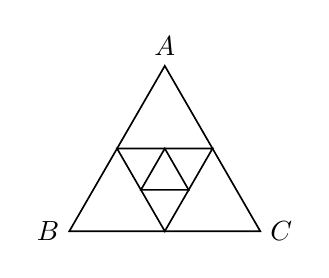
\begin{tikzpicture}[>=latex,scale=0.7]
  \draw[semithick](90:2)node[above]{$A$}--(210:2)node[left]{$B$}--(330:2)node[right]{$C$}--cycle;
  \draw[semithick](150:1)--(270:1)--(30:1)--cycle;
  \draw[semithick](90:0.5)--(210:0.5)--(330:0.5)--cycle;
\end{tikzpicture}
\end{document}